\subsubsection{Aufbau des Plugins}

Das Plugin kann in drei Hauptkomponente aufgeteilt werden:

\begin{itemize}
    \item \textbf{Plugin API:} Bildet die Schnittstelle zwischen der Capacitor Anwendung und dem Capacitor-NodeJS Plugin.
    \item \textbf{Implementierung:} Zuständig für den Start einer Node.js Runtime sowie für die Kommunikation zum Node.js Prozess.
    \item \textbf{Node.js Runtime:} Verantwortlich für die Ausführung des Node.js Projektes bzw.\ des JavaScript"=Codes.
\end{itemize}

\vfill

\begin{figure}[H]
    \centering
    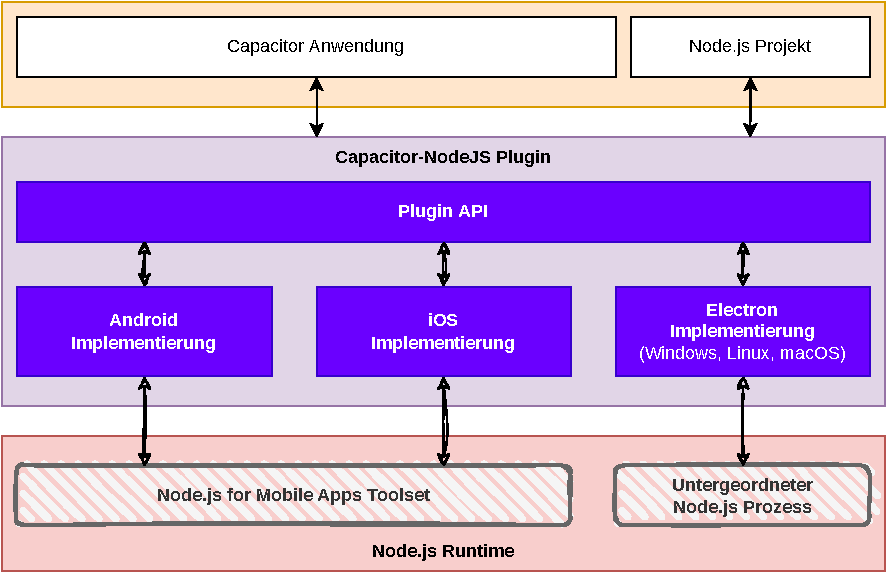
\includegraphics[width=\textwidth]{assets/02_Capacitor-NodeJS/02_Aufbau.drawio.pdf}
    \caption[Capacitor-NodeJS / Aufbau]{Aufbau des Capacitor-NodeJS Plugins}
\end{figure}

\vfill